\section{Waves in geosciences}
From the ripples on a water puddle to large breaking waves on the beach, we have all seen waves. 
They can be familiar or threatening, possibly deadly for seasoned fishermen or yachtsmen 
\citep[e. g. ][]{Pierson1972,Greenslade2001b}. Waves can exert huge forces: just try to stand up in the surf,
in front of a two-meter tall wave that breaks. And two meters is a far cry from the maximum recorded wave height at sea, towering
32~m above the following crest \citep{Liu&al.2008b}. The most severe \textit{sea state}, estimated from satellite radar altimetry, had a significant 
wave height of 20.1~m \citep{Hanafin&al.2012}, which, as we shall see in this chapter, 
means that some wave heights probably exceeded 35~m. Surfing contests have also focused on some specific coastal areas where waves are strongly amplified and produce waves of 30~m height or more, such as in Nazare, Portugal.

Knowing and predicting the properties of waves is necessary for sea-going operations, the design of any marine structure such as 
a jetty, an offshore platform or a ship. 
Waves modify the fluxes of momentum between the ocean and atmosphere and thus influence more or less directly the oceanic and 
atmospheric circulation. Waves are also an important agent in the pick-up and transport of sediments, and 
the main source of background seismic motions. 

%%%%%%%%%%%%%%%%%%%%%%%%%%%%%%%%%%%%%%%%%%%%%%%%%%%%%%%%%%%%%%%%%%%%%%
\begin{figure}[htb]
\centerline{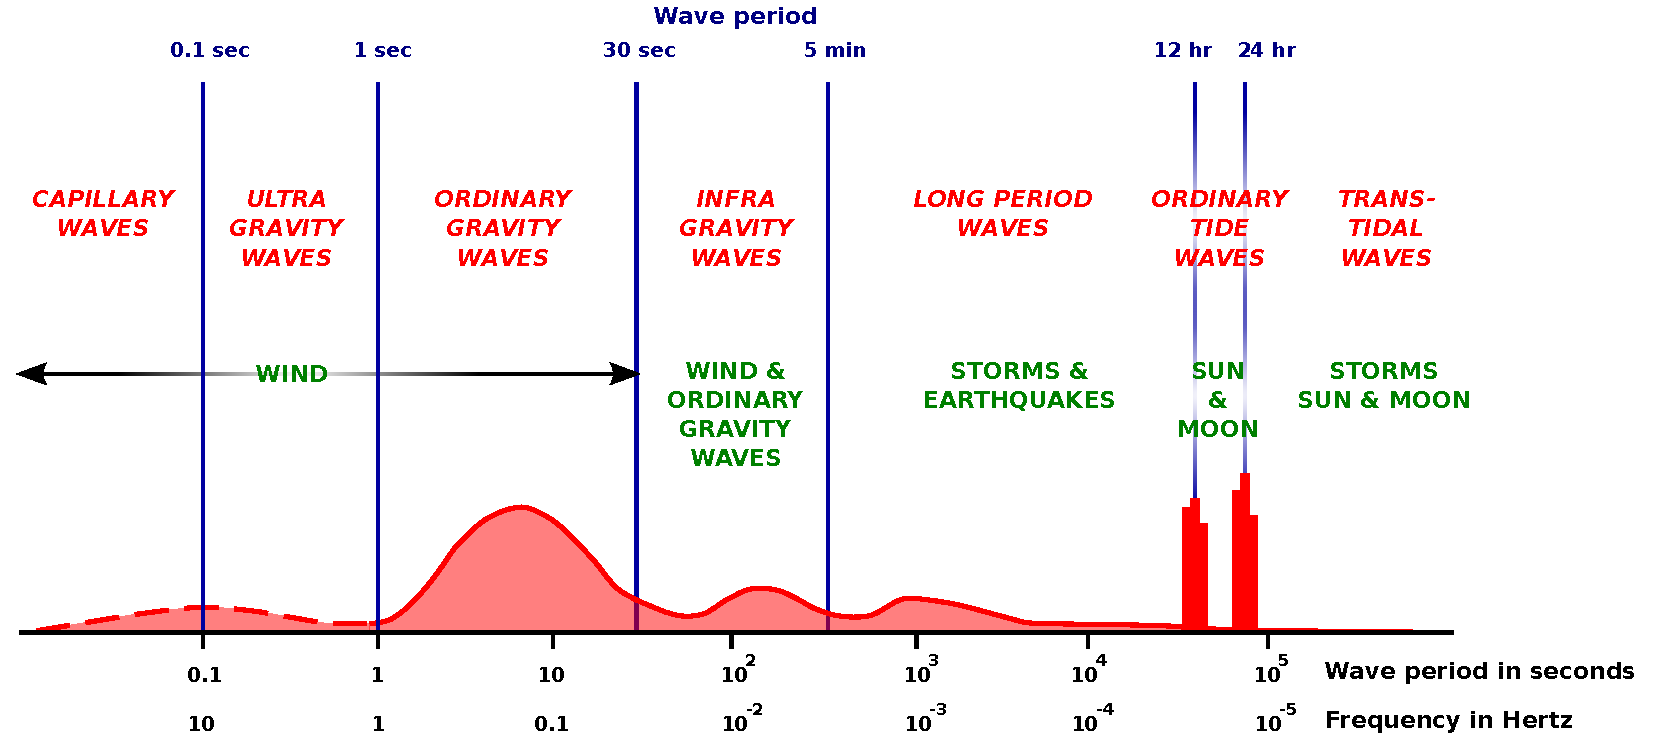
\includegraphics[width=\textwidth]{FIGS_CH_INTRO/Munk_ICCE_1950_Fig1.pdf}}
%\vspace{3.64in}
  \caption{Classification of the spectrum of ocean surface waves according to wave periods, forcing mechanisms and restoring force.}{Adapted from \cite{Munk1950}.}
\label{fig:Munk1950}
\end{figure}
%%%%%%%%%%%%%%%%%%%%%%%%%%%%%%%%%%%%%%%%%%%%%%%%%%%%%%%%%%%%%%%%%%%%%%%%%
To be more precise, we need now to introduce some classification of the different wave motions. A simple classification, as proposed by 
\cite{Munk1950} and shown in figure \ref{fig:Munk1950}, is based on the typical time scales of between the passing of two crests. We shall call this time scale the wave period and denote it with the symbol $T$, even though the motion does not repeat itself exactly and is not mathematically speaking periodic. 

Figure \ref{fig:Munk1950} has boundaries between capillary waves, ultra gravity waves, ordinary gravity waves, infragravity waves and longer period waves (including tides) at periods of 0.1, 1, 30, and 300~s. Most of this book will focus on "ordinary gravity waves" with periods 1 to 30~s. As a physicist by training, I've never liked classifications with dimensional quantities that are often used in natural sciences: these distinction are practically useful but they can be misleading.  Indeed, in some circumstances I would like to call "infragravity waves" some waves of periods around 10~s because they are generated by the same process as the usual waves with a period of 100~s. 

This period classification is closely related to a physical classification that distinguishes 
between the different  "restoring forces" which pulls back the surface towards a flat state, and the different generation processes for these waves. 
The two main restoring forces that we will consider are  \textbf{surface tension}, and \textbf{gravity}. Surface tension is mostly relevant for wave periods under 0.1~s, and will not be discussed much in the present book. Similar effects are produced by an ice layer that can be important for longer waves (their length depending on the ice thickness).

Once the restoring force is known, the next important things for any wave phenomenon are their
\begin{itemize}
          \item \textbf{generation},
          \item \textbf{propagation} 
          \item and \textbf{dissipation}.
         \end{itemize}
The goal of the present book is to describe and make understandable these 
three aspects, both qualitatively and quantitatively. 
This quantitative understanding allows an accurate forecast of local wave statistical properties, which we will 
call the sea state, as well as fluxes of energy and momentum between the atmosphere, ocean, sea ice, and solid Earth. 


In this book, we will restrict ourselves to waves which are more or less directly generated by the wind, leaving out 
tsunamis or ship wakes. But before leaving them out, let's say a few words about tsunamis. Tsunami propagation and dissipation properties 
are the same as the wind-waves described here, but whats sets them apart from wind-waves is their very large wavelength, 
which cannot be generated by wind in the same way as the usual wind-waves. Hence their generation mechanisms are specific, namely earthquakes, 
landslides, and meteorite 
impacts, which are all important but rare events, leading to very different statistical properties compared to the waves continuously 
generated by the wind. Another slightly more common source of meteo-tsunamis are abrupt changes in wind properties. 
All these generation events are transient, and typically cause a depression or bump of the sea surface that appears very fast but on a very 
large scale. This depression or bump then radiates a train of waves, with a period of the order of 10 minutes that is given by the size 
of the initial surface perturbation. These waves are strongly amplified in shallow water. The first perturbation to arrive on land can be a trough. 
If you see the sea retreating rapidly, this is it ... do not rush out to pick up crabs, but instead run to high ground, as a big crest will 
likely follow and flood what was the dry land. 

Instead of these transient wave trains, wind-generated waves are incessant and irregular.
The  time between the passing of two crests, which we define as the period $T$,  is typically less than 30~s. This limit is related 
to wind speeds, as explained in chapter \ref{ch_evol_profond}. 
These wind-waves also give rise to infra-gravity waves of periods 10~s to 10~minutes. For all these motions 
the average distance between two crests, which we shall call the mean wavelength $L_m$, increases with the mean period $T_m$. 
This wavelength goes from a few centimeters to about a kilometer. For wave shorter than a few centimeters, the effect of surface 
tension must be taken into account, and these short waves are called gravity-capillary waves. 

Indeed, the \textbf{propagation} properties of waves is related to the balance of forces near the air-sea interface. If gravity or surface tension is the dominant force then the propagation is different.
Gravity fights against surface slopes, setting up a pressure gradient that tends to reduce the sea level slope and is the main force 
for large wavelengths. Surface tension, instead, fights against surface curvature:
it arises from the difference in thermodynamic properties of the interface between the two fluids, that are air and water. 
This difference gives an energy to their interface, which is proportional to the area of the interface: the more curved the surface the 
larger the energy, which is the equivalent of the gravitational potential energy. This force explains 
why water droplets are spherical, it is simply the geometry that minimizes the area (hence the energy) for a given volume. 
This surface tension also explains why short breaking waves are not energetic enough to generate bubbles and foam at the sea surface. 
The presence of a continuous layer of ice can also act like an elastic layer with an effect similar to surface tension. In this case
even long waves can be influenced by the elasticity of the ice layer, this influence depends on the ice thickness \citep[e.g.][]{Squire&al.1995}. 
Because curvature is the second derivative of the surface elevation, surface tension effects is much stronger than gravity for small scales. 

Whether gravity or surface tension is the main restoring force, the work of these forces produces a motion with an associated kinetic energy. 
The oscillations of the air-sea interface are thus maintained by an exchange between potential and kinetic energy, 
until this energy is \textbf{dissipated}. Our waves are thus surface gravity waves, gravity-capillary or capillary waves for the shortest. 

In the family of gravity waves, at the other extreme towards the large scales, the slow oscillations on time scales of several hours to several days 
are also influenced by 
the Coriolis force, caused by the rotation of the Earth, and the waves become inertial-gravity waves, also known as Kelvin and Poincar{\'e}
waves. The main \textbf{generation} forces for these are the wind and the difference in the gravitational pull exerted by the Moon and Sun on the 
center and the surface of the Earth. Kelvin waves share many properties of gravity waves.

%%%%%%%%%%%%%%%%%%%%%%%%%%%%%%%%%%%%%%%%%%%%%%%%%%%%%%%%%%%%%%%%%%%%%%
\begin{figure}
\centerline{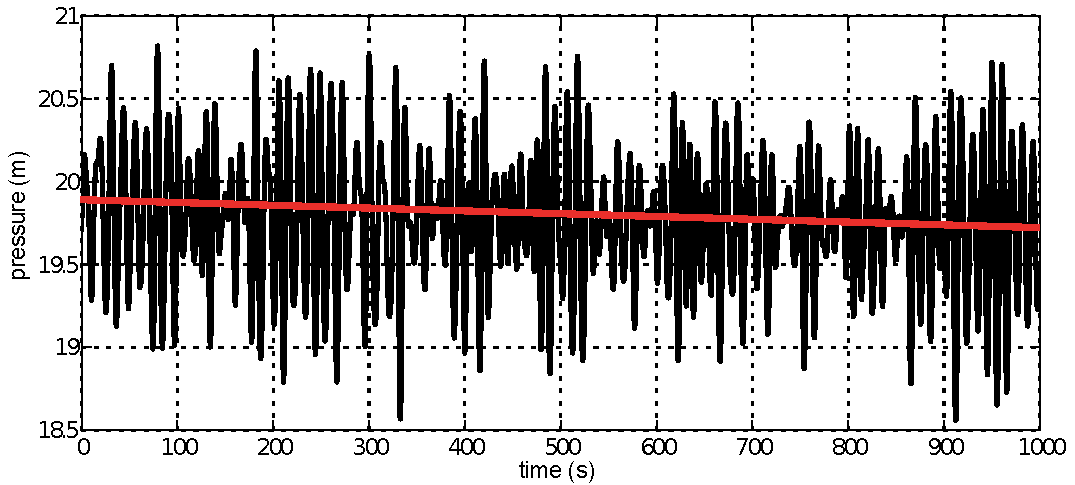
\includegraphics[width=\textwidth]{FIGS_CH_INTRO/p_at_berth1_en.pdf}}
%\vspace{3.64in}
  \caption{Example of the evolution of the bottom pressure in about 20~m of water 
 in Bertheaume bay, France, on January 31, 2004.}{The pressure in Pascals was converted here to an equivalent water height in meters
by dividing the absolute pressure 
recorded by a Nortek Vector %Seabird 26 
instrument, by the product $\rho_w g$ of water density $\rho_w \simeq 1026$kg/m$^3$, 
and gravity $g\simeq 9.81$m/s$^2$, after subtracting the atmospheric pressure recorded nearby, $p_a \simeq 10^5$Pa.  The 
fast oscillation caused by a swell of significant wave height $H_s=2.85$~m is superimposed on the tide 
that is gently falling, about 20~cm in 20~minutes, as shown by the red line.}
\label{pexemple}
\end{figure}
%%%%%%%%%%%%%%%%%%%%%%%%%%%%%%%%%%%%%%%%%%%%%%%%%%%%%%%%%%%%%%%%%%%%%%%%%

In practice, all these waves co-exist. Fortunately, it is often easy to sort them out and study them separately. 
Wind-waves and tides have very different periods and wavelengths, as illustrated by figure 
\ref{pexemple}. There is no such clear separation between capillary and gravity waves, except at low wind speeds 
when there is clear gap in the wave spectrum around the wavelength of 1.7~cm. For waves longer than 20~cm, 
we will ignore the effect of the surface tension which will greatly simplify our calculations. 
However, surface tension should not be ignored in general, in particular when considering 
wave dissipation by breaking and the effects of small scale surface roughness, both important for air-sea fluxes and remote sensing 
of the ocean surface.

The \textbf{propagation} of waves are generally well known thanks to the works of Laplace, Poisson, Stokes, Airy, Rayleigh and Boussinesq in 
the 18th and 19th centuries, with many later refinements. For a historical perspective, you may read the works of  \cite{Darrigol2003} and \cite{Craik2004}, and specific problems and questions are still open. The questions of  \textbf{generation} and \textbf{dissipation} are very active
research topics, with a fundamental problem posed by the multi-scale nature of real ocean waves: how short waves influence long waves and vice versa is 
very difficult to measure and analyze. Because of the strong demand for results, successful forecasting methods have been developed on more or less empirical grounds. 
Modern wave forecasting started with swell forecasts
for Morocco, in the 1920s \citep{Gain1918,Montagne1922}. This approach was generalized by 
\cite{Sverdrup&Munk1947} who considered the full life cycle of waves, from generation by the wind to dissipation 
in the middle of the ocean and on beaches. This latter work was 
motivated by the planning of the allied amphibious operation Torch in Morocco in 1942, which led to a method later applied to Normandy 
and many Pacific islands. Their British colleagues, forming the W group at the Admiralty, included Deacon, Darbyshire, Barber, Ursell and Longuet-Higgins  
who developed similar methods and introduced the spectral analysis of waves in 1945 \citep{Ursell1999}, paving the way for 
today's numerical wave models. The first numerical spectral wave model was developed by \cite{Gelci&al.1957}, the group that continued the Morocco wave forecasting effort in Casablanca.


Today, we can forecast with good confidence the main properties of the sea state and its consequences, including forces on a structure 
at sea, ship motions, working range of a radar... although the details of the generation and dissipation processes are not well known. 
This is a tribute to the flair of those who invented rules and equations to represent the complex and poorly known reality. 
However, given this empirical part, it is not surprising that the same models may not be accurate for secondary properties of the sea state, such as the distribution 
of the energy radiated in different directions or the statistics of short breaking waves. 


Going against the long-term specialization and separation of geosciencies in many sub-disciplines, 
there has been a strong interest since the late 1990s in the interaction of waves with the atmosphere, ocean currents, 
turbulence, sediment motion, from the scale of the global ocean to the small scale of any particular beach. This is motivated by 
integrated approaches for climate projections or the understanding of sediment transport from sources to sinks. 
These efforts should be continued to properly understand the interactions of waves and turbulence, and the multi-scale 
properties of the ocean surface. 
We hope that after reading the present book, that gives a broad view of what is known and tries to highlight what is still unclear,
the reader will gather the courage to continue the exploration of ocean waves after Stokes, Boussinesq, Munk, Longuet-Higgins,
Hasselmann, Zakharov, Katsaros, Phillips and many other less famous scientists who made today's knowledge possible. 

Courage, though, may not be enough, and some tools will be needed to start for this journey, including 
a working knowledge of calculus and fluid mechanics. 

The following books should be consulted for complements on different topics, 
\begin{itemize}
\item \cite{Kinsman1965} on general principles and wave measurements, in particular with arrays of sensors. Although a bit 
old, this book is very well written and easy to get into. 
\item \cite{Phillips1977} for a comprehensive view, although not up to date, of upper ocean processes (waves, internal waves, turbulence ...) 
\item \cite{Mei1989} for wave propagation, mass transport and wave-structure interactions
\item \cite{Dean&Dalrymple1991} gave a real textbook oriented towards engineering applications
\item \cite{WAMBook} gives the fundamental -- but not basic -- concepts of numerical wave prediction 
in the open ocean, this is not an easy read
\item \cite{Komar1998} wrote a nice textbook for coastal geomorphology, an excellent starting point for those 
who do not have a strong physics background
\item \cite{Young1999}  combined deep and shallow water waves, including also global wave climatology. 
\item the Coastal Engineering Manual \citep{USACE2002}, replaced the Shore Protection Manual. This book 
is edited by the U.S. Army Corps of Engineers, the body in charge of shoreline defenses and management of 
ports and waterways. This combines general principles with empirical formulas for coastal engineering. This is 
freely available on the web. 
\item \cite{Janssen2004} give the ECMWF perspective on wind and wave forecasting, with many theoretical details on wind-wave 
generation and nonlinear wave evolution. 
\item \cite{Holthuijsen2007} A very well illustrated textbook centered on numerical wave modelling, specifically for coastal 
environments, although a bit weak on physical processes, such as bottom friction.  
\end{itemize}
A lot of interesting material and teaching aids can be found on the web, from Tony Dalrymple's Java applets, to the UCAR Meted program 
targeted at meteorologists. A list of useful links will be proposed separately for each chapter. 

Let us now beg the tides and currents to stop their flow, so that we may study waves quietly. We will see later, in chapters \ref{ch_courant} and 
\ref{ch_littoral} how waves interact with other oceanic motions. 

\section{Wave motion: some observations}
The random nature of ocean waves has long puzzled observers and made difficult all scientific investigations. 
Figure \ref{pexemple} gives a good example of a random sequence of high and low waves. Initially  
the forecasting of waves was formulated in terms of the highest wave. The notion of wave height distribution was only introduced after 1945, 
thanks to the development of wave recording devices, and the availability of computing power. Two types of methods have been developed to 
represent the random nature of the wave field. 
One of these is the spectral analysis, which will be heavily used in the following chapters. The other, is the wave-by-wave analysis, 
which we briefly describe here. More recent time-frequency analyses are a kind of hybrid of these two methods. 


Both methods are very useful and have their own limitations. Spectral analyses is well suited for the wave forecasting, in 
particular at large scales, because it explicitly represents the dispersion of waves that have different periods. 
Spectral analysis decomposes the sea surface in elementary sinusoidal waves, it is thus very important to know the properties of these 
sinusoidal waves. This is the topic of chapter \ref{ch1b}.
However, some sort of wave-by-wave analysis must be use to investigate localized 
events associated to the finite amplitude of the waves, such as breaking, as discussed in section
\ref{section_whitecap} and chapter \ref{ch_sds}. 

%%%%%%%%%%%%%%%%%%%%%%%%%%%%%%%%%%%%%%%%%%%%%%%%%%%%%%%%%%%%%%%%%%%%%%%%%%%%%
\begin{figure} \label{FigWaveriderTSz}
\centerline{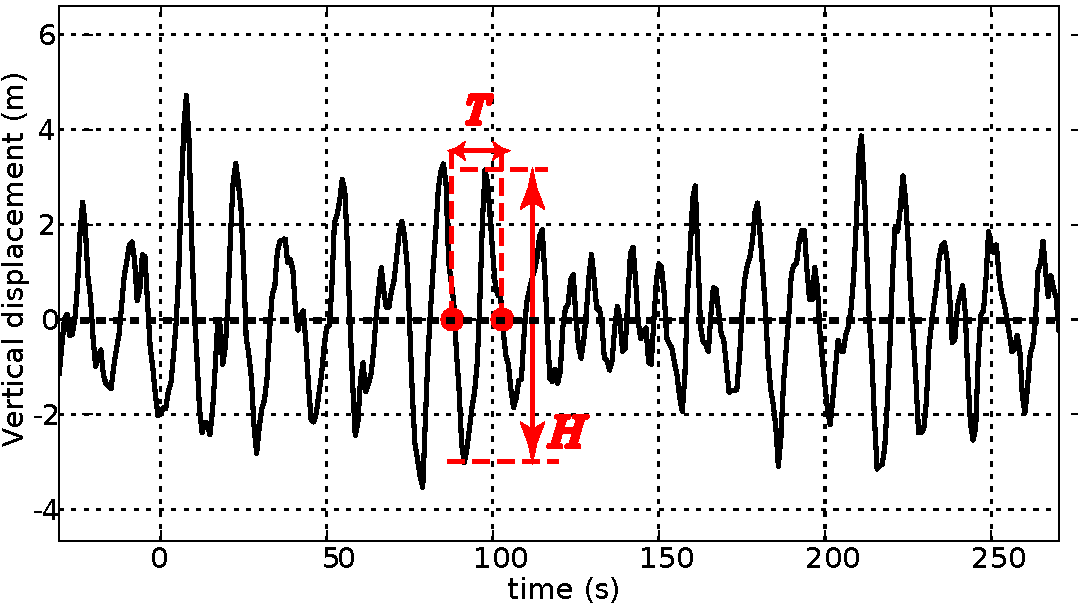
\includegraphics[width=0.8\textwidth]{FIGS_CH_INTRO/Exemple_DWIROISE2004_en.pdf}}
%\vspace{3.64in}
  \caption{Principle of wave by wave analysis: a series of elevation records is broken in individual waves of duration $T$. The separation from one 
wave to the next is the zero down-crossing of the vertical displacement. This example was obtained from a Datawell Waverider buoy deployed offshore 
of Crozon, France, in May 2004.}\label{fig:zero_crossing}
\end{figure}
%%%%%%%%%%%%%%%%%%%%%%%%%%%%%%%%%%%%%%%%%%%%%%%%%%%%%%%%%%%%%%%%%%%%%%%%%%%%%


\section{Wave-by-wave analysis\label{anavague}}
\subsection{Time series}
Time series are the most common type of measurement these days, let us see what we can learn about waves from time series. 
We shall work with series of sea surface elevation, but we could have used any other physical quantity such as the 
velocity or pressure in the water or in the air. 

We first define a single wave in time series by the time interval between two consecutive 
crossings of the mean sea level as the surface goes down, as illustrated in Fig. \ref{fig:zero_crossing}. 
The choice of 'down' instead of 'up' is fairly arbitrary but it 
keeps the forward face of the wave, which is usually  more interesting, within a single wave, whereas the rear face is split 
between two consecutive waves. 
For each wave we define a period $T$, which is the length of the time interval, and a height $H$, which is the 
difference between the maximum elevation (the crest) and the minimum elevation (the trough) during the perid. 



From a sequence of heights, we can define a probability density function (PDF) $dP$ as the limit, when $dH$ 
goes to zero, of the probability $P$ that a wave height is between $H$ and $H+dH$, divided by $dH$. 
For a statistically stationary sea state, the surface elevation is well approximated by the sum of  a large number 
of sine waves which are independent from one another. Applying the central limit theorem to this 
approximate model, we find that the surface elevation is a Gaussian process, with negative and positive anomalies around the mean sea level 
with statistics defined uniquely by the standard deviation of the sea surface elevation. As a result, and this was proven in the narrow frequency band limit 
by \cite{Rice1944} and \cite{Cartwright&Longuet-Higgins1956}, the heights follow a Rayleigh distribution, as shown on figure \ref{fig:Rayleigh}, 
 \begin{equation}
dP(H)=\frac{2H}{H_{\mathrm{rms}}^2}
\exp^{-{H^2}/{H_{\mathrm{rms}}^2}}.
\end{equation}
This PDF is normalized to give 
$\int_0^\infty dP dH =1$. The Rayleigh distribution is generally a good approximation for 98\% of the distribution, sometimes even more. 
For extreme values, a better approximation was given by \cite{Tayfun1980}, taking into account the correlations among wave components due to 
second-order nonlinearities. 
%%%%%%%%%%%%%%%%%%%%%%%%%%%%%%%%%%%%%%%%%%%%%%%%%%%%%%%%%%%%%%%%%%%%%%%%%%%%%
\begin{figure}
\centerline{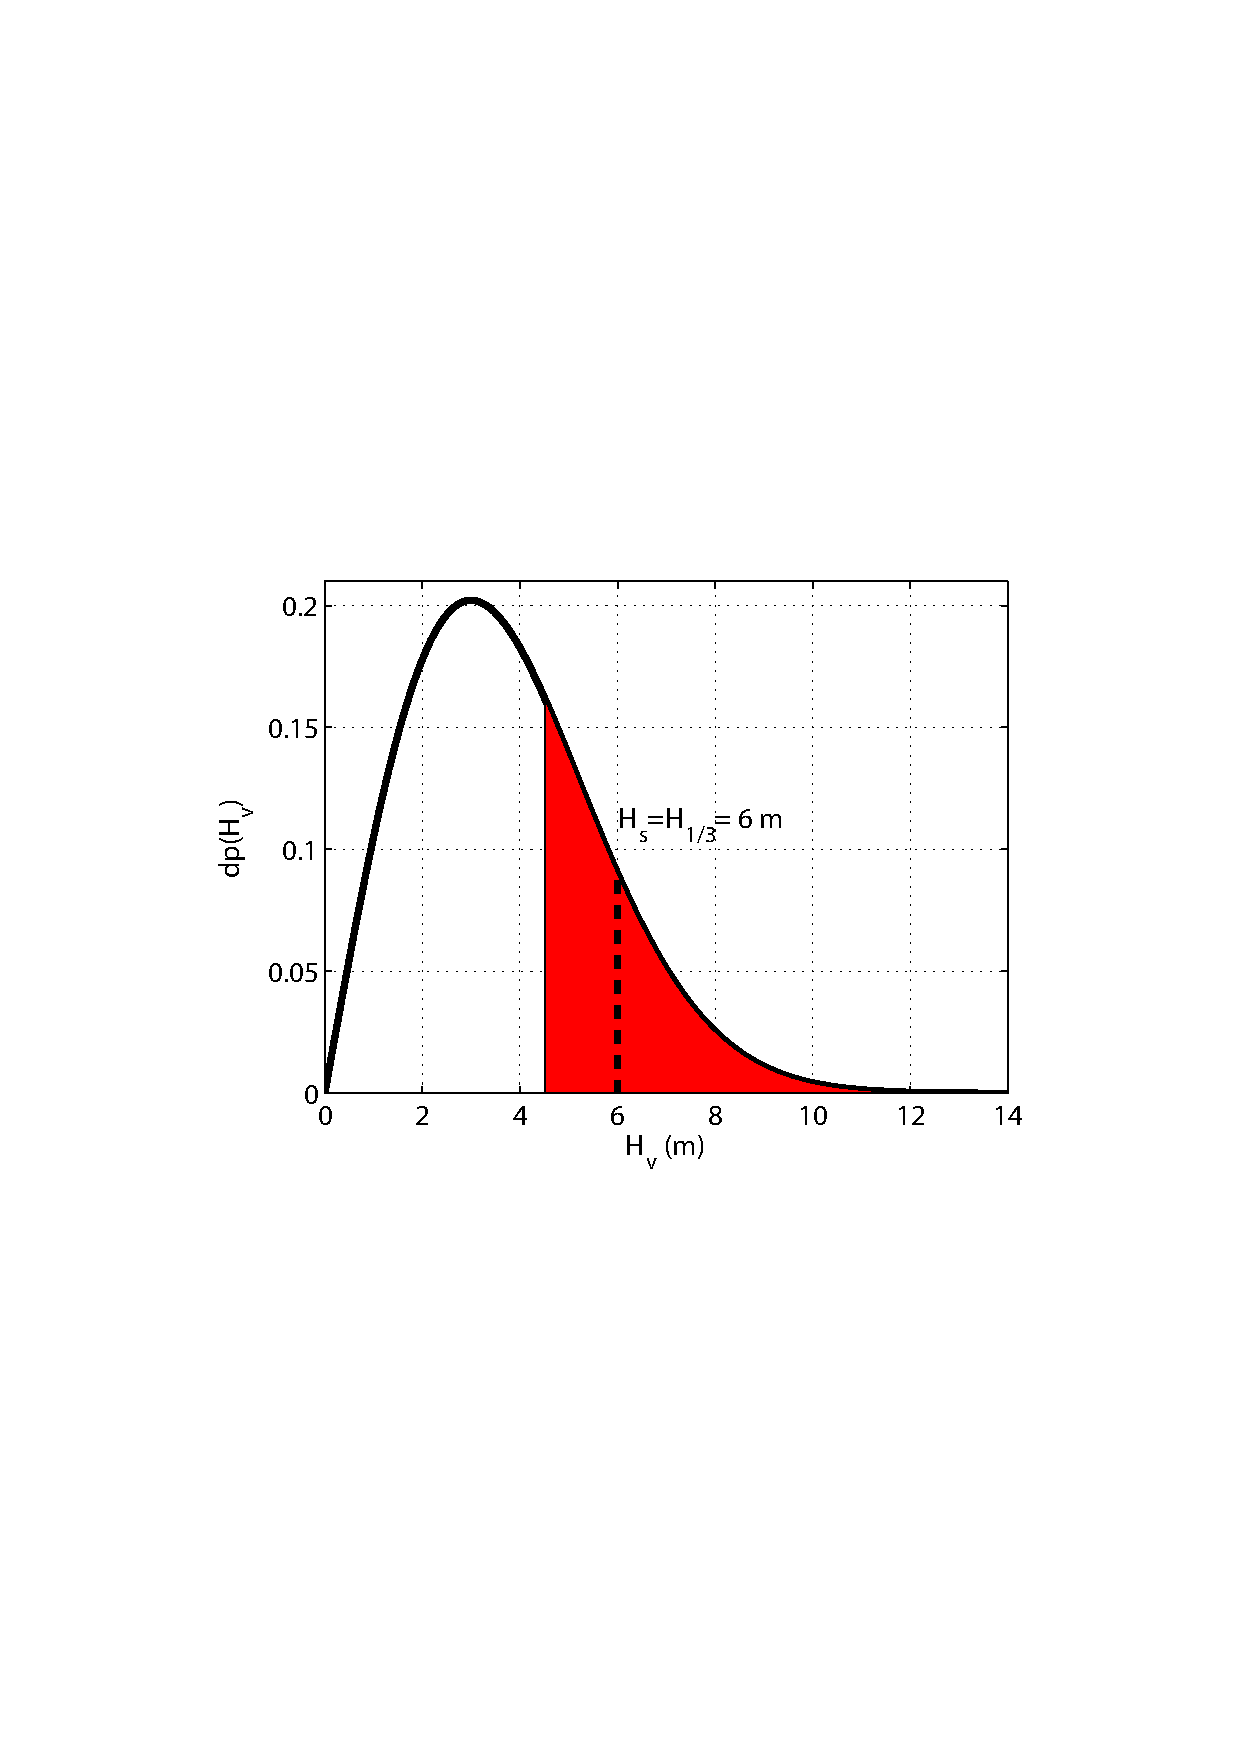
\includegraphics[width=0.6\textwidth]{FIGS_CH_INTRO/Rayleigh.pdf}}
%\vspace{3.64in}
  \caption{ Rayleigh distribution of wave heights}{$dp\times dH(H_v)$ is a probability for a single wave to have a height between  $H_v$ and $H_v+dH$. 
In red: the 1/3 of the highest waves in the distribution. The average height in this red part is $H_{1/3}$, which is one way to define the  significant wave height $H_s$. 
In the following chapters we will rather define $H_s$ as $H_{m0}$, equal to four times the standard deviation of the sea surface elevation. That other definition is 
recommended by the World Meteorological Organization and it gives a number 
very close to $H_{1/3}$.\label{fig:Rayleigh}}
\end{figure}
%%%%%%%%%%%%%%%%%%%%%%%%%%%%%%%%%%%%%%%%%%%%%%%%%%%%%%%%%%%%%%%%%%%%%%%%%%%%%

One useful result is that the probability that the height exceeds a given threshold $\widehat{H}$ 
is given by 
 \begin{equation}
P(H
>\widehat{H})=\er^{-\left(\widehat{H}/H_{\mathrm{rms}}\right)^2}\label{Hseuil}.
\end{equation}
This expression can be used to compute the height threshold $\widehat{H}$
associated to a fixed fraction of the wave population. For example 
$\widehat{H}_{1/3}$ is the height beyond which there are the highest 1/3 of the waves, and it is 
 $\widehat{H}_{1/3}=\left(\ln(3)\right)^{1/2}
H_{\mathrm{rms}}$ which is nearly 1.05$\times H_{\mathrm{rms}}$. 

A more widespread scale for the wave heights is given by integrating 
 (\ref{Hseuil}) to get the average height of the 1/3 highest waves. This is one definition of 
the significant wave height, denoted $H_{1/3}$ or $H_s$. This scale roughly corresponds to the visual impression of wave heights, which was the most common source 
of measurements until the 1940s. 
More generally but still for a Rayleigh distribution, the average height of the $1/x$ fraction of the highest waves is, 
\begin{equation}
\left[\left(-\ln(1/x)\right)^{1/2} + \sqrt{\pi} \times
{\mathrm{erfc}}\left[\left(\ln(x)\right)^{1/2}\right]/2\right]
H_{\mathrm{rms}}
\end{equation}
 where erfc is the complementary error function.  For 
$x=1/3$, this gives $H_{1/3}=1.4157 \times H_{\mathrm{rms}}$.

From the definition, the full Rayleigh PDF $p(H)$ is determined by $H_{\mathrm{rms}}$. In practice the average $H_{1/3}$ is more 
commonly used, and there is also a lot of interest in the maximum height $H_{\mathrm{max}}$, but that one depends on the length of the 
record. When recording more waves,  $H_{\mathrm{max}}$ is likely to be higher. Waves that have a height
$H$ larger than $2.1 H_{1/3}$ are called freak waves or rogue waves. If we follow the Rayleigh statistics, 
this correspond to 1 in 5700 waves. In practice, they are a bit more frequent for conditions with large average steepnesses, as 
predicted by \cite{Tayfun1980}. Also, for real waves the spectrum is not always narrow and on average $H_{1/3} \simeq 3.8 \sqrt{m_0}$
instead of $H_{1/3} \approx 4.004 \sqrt{m_0}$, where $m_0$ is the variance of the surface elevation \citep{Goda1985}.

In the context of the design of coastal or oceanic structures,  there is a great interest in defining the 
maximum wave conditions that will occur over the expected lifetime of a structure, typically 50 to 100 years, 
or with a very low probability of occurrence to ensure maximum safety. For example, some sections of the Dutch dyke system
are required by law to resist waves that occur only once in 10,000 years. 
The material and size of the structure is then designed to withstand 
these extreme conditions. If the extreme wave height and period is overestimated, the cost of construction 
is higher than it could have been. If the conditions are underestimated, the structure is likely to fail in a time shorter
than the expected lifetime. This early failure happened for the first oil platforms built in the North Sea, in an age
when there were no routine wave measurements. 

For these extremes, the Rayleigh distribution does not hold, because the $H_s$ is itself a random variable on the 
scale of days to centuries. The extreme wave statistics on these long time scales are determined by the 
distribution of extreme meteorological event, or, in shallow water, the joint distribution of water levels (including 
the astronomical tide) with weather events. These long term statistics are clearly different from the short term statistics. 
For short term, the sea state was a superposition of many independent wave trains, and we could use the central limit theorem. 
For long terms, we first need to determine the distribution of the significant wave heights  $H_{s}$, and the probability 
that the height of a single wave exceeds $H_0$ is then the conditional 
probability $p(H > H_0  | H_s = H_{s0})$. The distribution of $H_s$ follows a generalized Pareto distribution, 
and the probability $p(H > H_0)$ is given by integrating the conditional probability over $H_{s0}$. 

Obviously, this requires stationary statistics. In some regions 
these statistics fluctuate with climatic patterns like the North Atlantic Oscillation, which particularly impacts
the wave heights on the European Atlantic coast, or the El Nino-Southern Oscillation  (ENSO) which has a strong 
impact on waves in the central Eastern Pacific or on the U.S. West coast \citep{Bromirski&al.2005}. 
As an example, Edward Thornton, a renown specialist of nearshore dynamics, was asked in 1996 to provide 
some consulting advice for the construction of a wastewater pipeline in Monterey Bay, Central California. 
Construction started in 1997 in the middle of a very strong El Nino, 
the hundred-year wave height, which had been properly evaluated by Ed Thornton, was exceeded 
and the half-ton rocks protecting the pipe were too small to stay in place and were dispersed by the waves. 
For such a strong El Nino event, the storm waves that caused the damage on the U.S. West Coast were normal. 
One should thus use statistics with caution. Defining extreme wave heights is also very challenging in tropical areas where
they are associated with hurricanes that have random tracks: a 20-year record of hurricane tracks generally does not contain 
all possible tracks, in particular the one of the next hurricane that will destroy this or that facility. 
Finally, there are also long-term trends associated with global change \citep[e.g.][]{Wang&Swail2002,Charles&al.2012}, 
especially in the Arctic where the trend in sea ice extent  is leading to higher wave heights and periods \citep{Stopa&al.2016b}. 

\subsection{Maps}
Wave statistics from time series cannot represent all wave properties. Some of these, such as the 
length of crests, are defined from the spatial 
patterns in the wave field. This parameter, although secondary to the wave height, gives information 
on the spatial coherence of wave-induced motions and is thus very important when navigating a seaway or designing 
a structure that may be wider than the crest length.
 
Just like we have defined heights and periods, heights and lengths $L$ can be defined 
in the case of waves propagating all in the same direction, say $x$. In that case, the crests are infinitely long in the other 
direction $y$. One important parameter is then the wave slope, defined from the ratio $H/L$. For sinusoidal waves, the maximum 
slope is $\pi H/ L$. 

Things get more complex when considering real waves that propagate in all directions. 
One can use the theory of random fields, developed by \cite{Adler1981}. In that theory, the crests are defined 
as subsets of the horizontal plane that are simply connected and that are above the mean sea level. Using this definition 
requires a bit of topology. In this context it becomes more difficult to associate a crest with a trough. 
There is a strong development of spatial statistics for ocean engineering and oceanography, thanks to the development 
of video measurement techniques \citep{Fedele&al.2009a}. 
